%%%%%%%%%%%%%%%%%%%%%%%%%%%%%%%%%%%%%%%%%
% Beamer Presentation
% LaTeX Template
% Version 1.0 (10/11/12)
%
% This template has been downloaded from:
% http://www.LaTeXTemplates.com
%
% License:
% CC BY-NC-SA 3.0 (http://creativecommons.org/licenses/by-nc-sa/3.0/)
%
%%%%%%%%%%%%%%%%%%%%%%%%%%%%%%%%%%%%%%%%%

%----------------------------------------------------------------------------------------
%	PACKAGES AND THEMES
%----------------------------------------------------------------------------------------

\documentclass{beamer}

\mode<presentation> {

% \usetheme{Madrid}

\setbeamertemplate{navigation symbols}{} % To remove the navigation symbols from the bottom of all slides uncomment this line
}

\usepackage{graphicx} % Allows including images
\usepackage{booktabs} % Allows the use of \toprule, \midrule and \bottomrule in tables
\usepackage{amssymb}
\usepackage{amsmath}
\usepackage{textpos}
% \usepackage{subfigure}
% \usepackage{cite}
\usepackage[T1]{fontenc}
\usepackage{subfig}
\usepackage{listings}
\usepackage{mathtools}

\newcommand{\p}{\text{p}}

\definecolor{gray}{rgb}{0.4,0.4,0.4}
\definecolor{darkblue}{rgb}{0.0,0.0,0.6}
\definecolor{cyan}{rgb}{0.0,0.6,0.6}

\lstset{
  basicstyle=\ttfamily,
  columns=fullflexible,
  showstringspaces=false,
  commentstyle=\color{gray}\upshape
numbers=right, 
                numberstyle=\tiny, 
                breaklines=true,
                numbersep=5pt,
                xleftmargin=.25in,
                xrightmargin=.25in
}

\lstdefinelanguage{XML}
{
  morestring=[b]",
  morestring=[s]{>}{<},
  morecomment=[s]{<?}{?>},
  stringstyle=\color{black},
  identifierstyle=\color{darkblue},
  keywordstyle=\color{cyan},
  morekeywords={xmlns,version,type}% list your attributes here
}

\DeclareMathOperator*{\argmax}{\arg\!\max}

\title[Automatic Metadata Extraction]{Automatic Metadata Extraction \\ The High Energy Physics Use Case} % The short title appears at the bottom of every slide, the full title is only on the title page

\author{Joseph Boyd} % Your name
\institute[EPFL] % Your institution as it will appear on the bottom of every slide, may be shorthand to save space
{
\'Ecole Polytechnique F\'ed\'erale de Lausanne \\ % Your institution for the title page
\medskip
\textit{joseph.boyd@epfl.ch} % Your email address
}
\date{\today} % Date, can be changed to a custom date

% \logo{
\includegraphics[height=1cm]{Figures/EPFL-logo.jpg} \ \ 
\includegraphics[height=1cm]{Figures/CERN-logo.jpg}}

\begin{document}

\begin{frame}
\titlepage % Print the title page as the first slide
\end{frame}

%------------------------------------------------

\section{Introduction}

%------------------------------------------------

\begin{frame}
\frametitle{Motivation}
\begin{itemize}
\item INSPIRE-HEP digital library at CERN contains over 1 Million documents
\item Manual curation of high energy physics (HEP) papers may be automated with machine learning techniques
\item Custom datasets and specialised features required to model HEP paper characteristics
\end{itemize}
\end{frame}

%------------------------------------------------

\begin{frame}
\frametitle{Aims}
Take existing state-of-the-art system for metadata extraction to:
\begin{itemize}
\item demonstrate a qualitative difference between HEP and general papers;
\item propose improvements to model features;
\item run experiments to confirm these improvements, and;
\item draw conclusions about what characterises good feature engineering.
\end{itemize}
\end{frame}

%------------------------------------------------

\section{Theory}

%------------------------------------------------

\begin{frame}[noframenumbering]{Outline}
\tableofcontents[currentsection, currentsubsection]
\end{frame}

%------------------------------------------------

\begin{frame}
\frametitle{Why CRFs?}
\begin{itemize}
\item Transition interdependencies implies graphical structure best modelled as a structured sequence
\item Modelling conditional distribution, $p(\textbf{y}|\textbf{x})$ sufficient for classification
\item Exploit rich information about observations, $\textbf{x}$, without explicitly modelling the underlying probability distribution
\item Classifying metadata may greatly benefit from modelling rich text features (punctuation, font size, layout,...)
\end{itemize}
\end{frame}

%------------------------------------------------

\begin{frame}
\frametitle{Mathematical Formulation}
\begin{equation}
\p(\textbf{y}|\textbf{x}) = \frac{\p(\textbf{x}, \textbf{y})}{\sum_{y'}{\p(\textbf{x}, \textbf{y}')}} = \frac{1}{Z(\mathbf{x})}\exp \Bigg\{\sum_k{
\lambda_{k}F_{k}(y_t, y_{t-1}, x_t)
}\Bigg\},
\end{equation}

where $Z(\mathbf{x}) = \sum_{y'}\exp \Big\{\sum_k{\lambda_{ij}F_{k}(y'_t, y'_{t-1}, x_t)}\Big\}$ is known as the partition function, ensuring probabilities sum to 1.

$F_k(\mathbf{x}, y) = \sum_t^T f_k(\mathbf{x}, y)$, where $f_k$ is a (typically boolean) function describing one of several features about a token.

The form of the functions themselves, $f(\cdot)$, are known in Wapiti (Section \ref{sec:wapiti}) as \emph{templates}. It is in choosing these explicitly that we perform feature engineering.
\end{frame}

%------------------------------------------------

\begin{frame}
\frametitle{Solution Approach}
\begin{itemize}
\item Formuluate convex maximum log likelihood estimator, $l(\Lambda)$, where $\Lambda = \{\lambda_k\}_{k=1}^K$
\item Train (determine $\Lambda$) with gradient ascent technique, L-BFGS. Each iteration, $I$, requires forward-backward algorithm to compute $Z(\mathbf{x^{(n)}})$ for each of $N$ samples -- $\mathcal{O}(INT|S|^2)$.
\item Prediction with Viterbi algorithm -- $\mathcal{O}(T|S|^2)$.
\end{itemize}
\end{frame}

%------------------------------------------------

\section{Automatic Metadata Extraction}

%------------------------------------------------

\begin{frame}[noframenumbering]{Outline}
\tableofcontents[currentsection, currentsubsection]
\end{frame}

%------------------------------------------------

\begin{frame}
\frametitle{Metadata Extraction}
\begin{itemize}
\item \emph{Metadata} refers to content useful to the identification of the document
\item \emph{Extraction} refers to the identification of metadata within the document text
\item Several automatic approaches exist: stylistic analysis, knowledge-base, machine learning, ...
\end{itemize}
\end{frame}

%------------------------------------------------

\begin{frame}
\frametitle{Metadata Extraction (Illustration)}
\begin{figure}[h]
\center
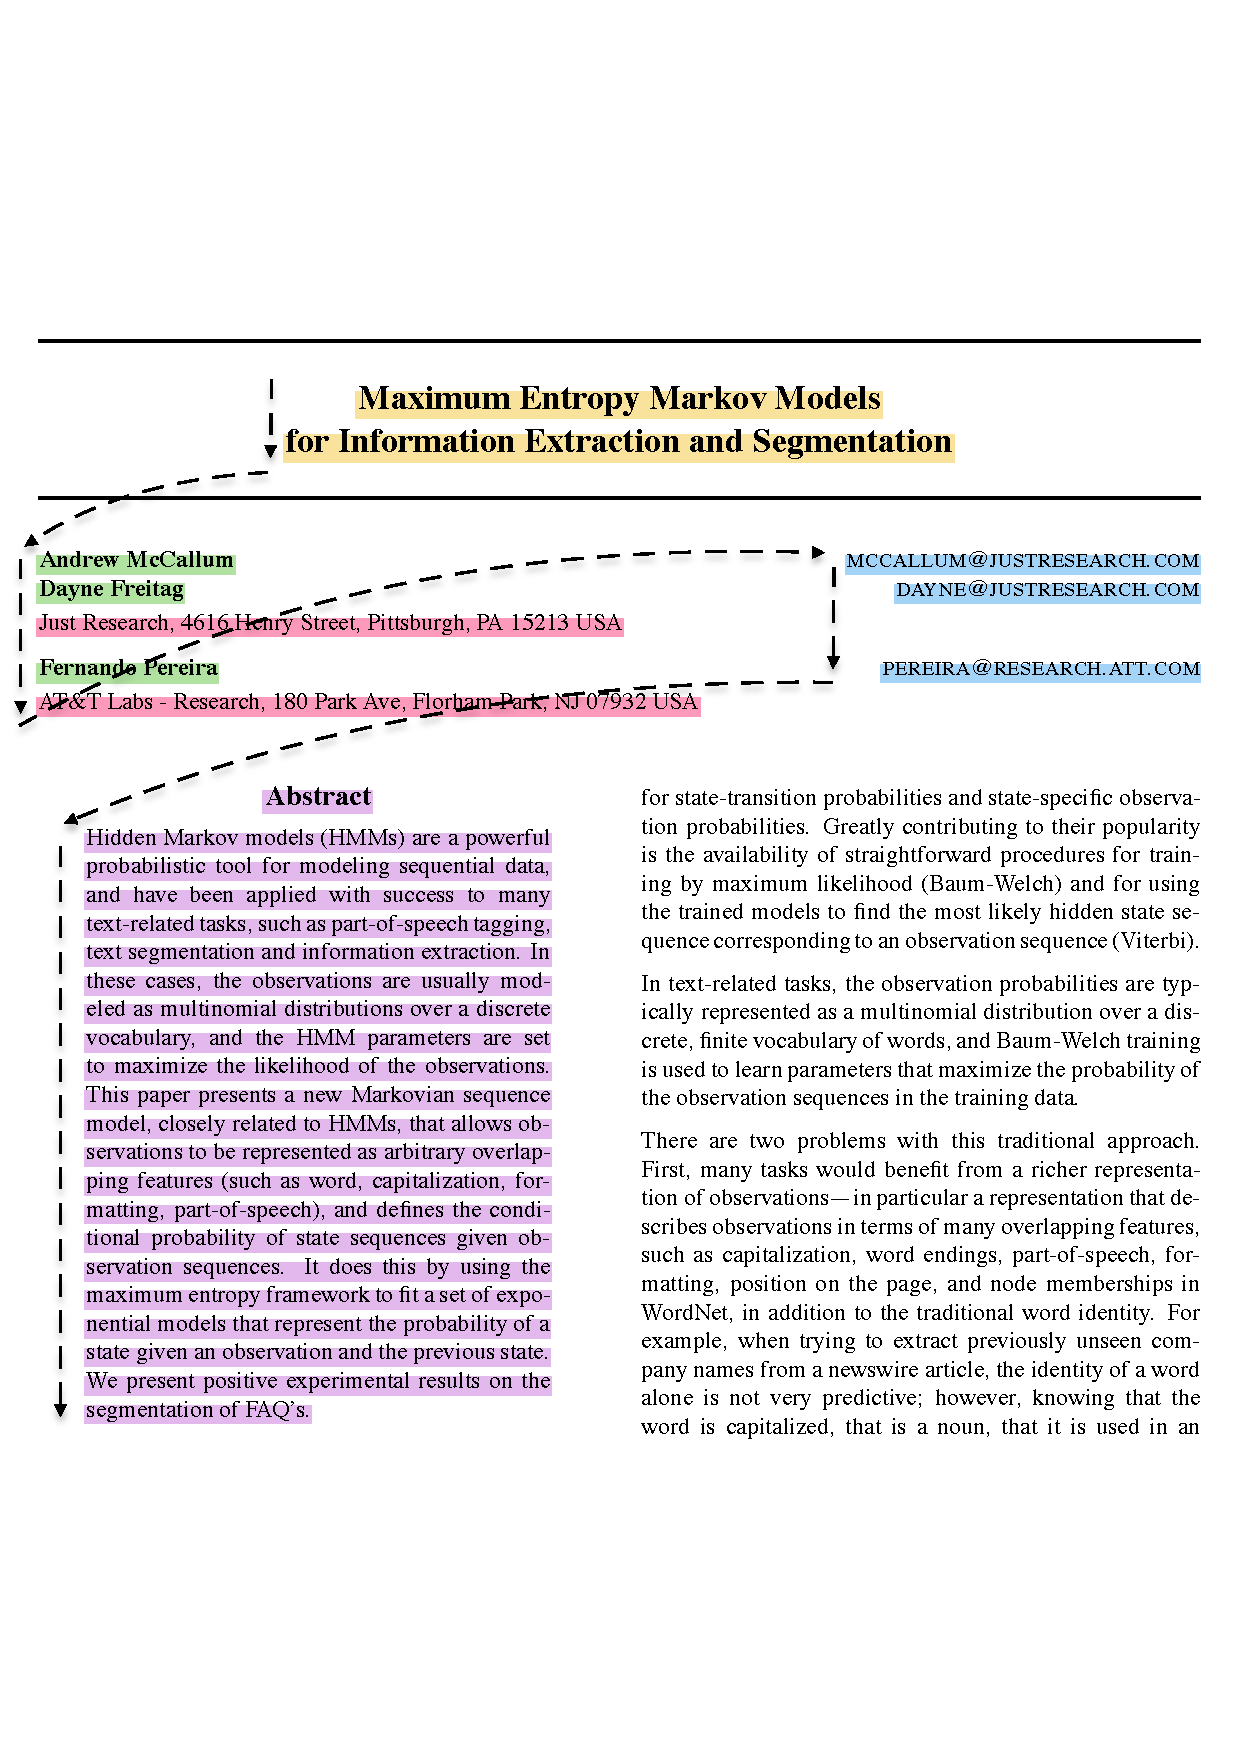
\includegraphics[width=3in]{Figures/extraction.pdf}
\caption{Tagging of a document header section.}
\end{figure}
\end{frame}

%------------------------------------------------

\begin{frame}
\frametitle{GROBID}
\begin{itemize}
\item Selected according to performance in study comparing AME systems \cite{
lipinski2013evaluation}
\item Open source Java-based tool developed at INRIA, France
\item Manages \emph{cascade} of CRF models for annotating papers in progressively finer detail
\item Uses C++ library \emph{Wapiti} for back-end calculations (training, prediction)
\end{itemize}
\end{frame}

%------------------------------------------------

\begin{frame}
\frametitle{GROBID - CRF Cascade}
\begin{figure}[h]
\center
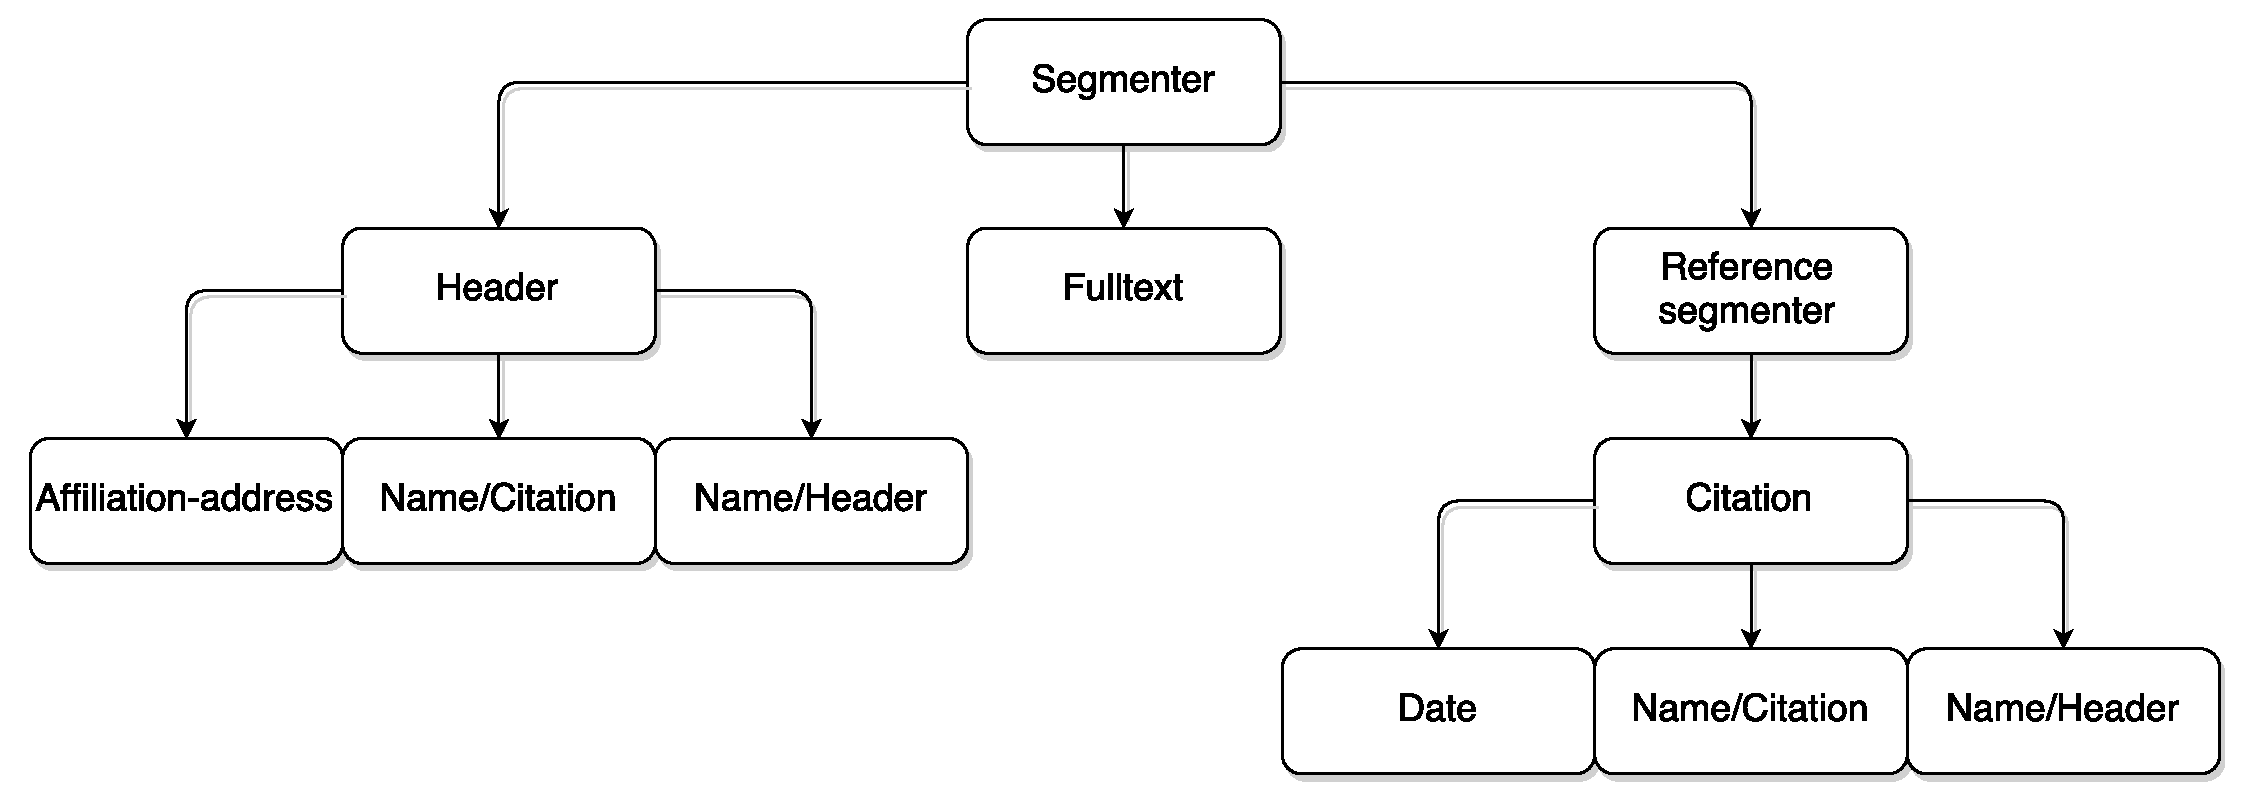
\includegraphics[width=4in]{Figures/cascade.pdf}
\caption{Cascade of models used by Grobid}
\end{figure}
\end{frame}

%------------------------------------------------

\section{Data, Methods, and Implementation}

%------------------------------------------------

\begin{frame}[noframenumbering]{Outline}
\tableofcontents[currentsection, currentsubsection]
\end{frame}

%------------------------------------------------

\begin{frame}
\frametitle{}
\begin{figure}[h]
\centering
\begin{tabular}{cc}
\subfloat[Collaboration field in header section.]{
\includegraphics[width=0.45\textwidth]{Figures/collaboration.pdf}}\label{fig:articlesamplesA}&
\subfloat[Discontinuous header data.]{
\includegraphics[width=0.45\textwidth]{Figures/eamonn.pdf}} \\
\subfloat[Collaboration author list.]{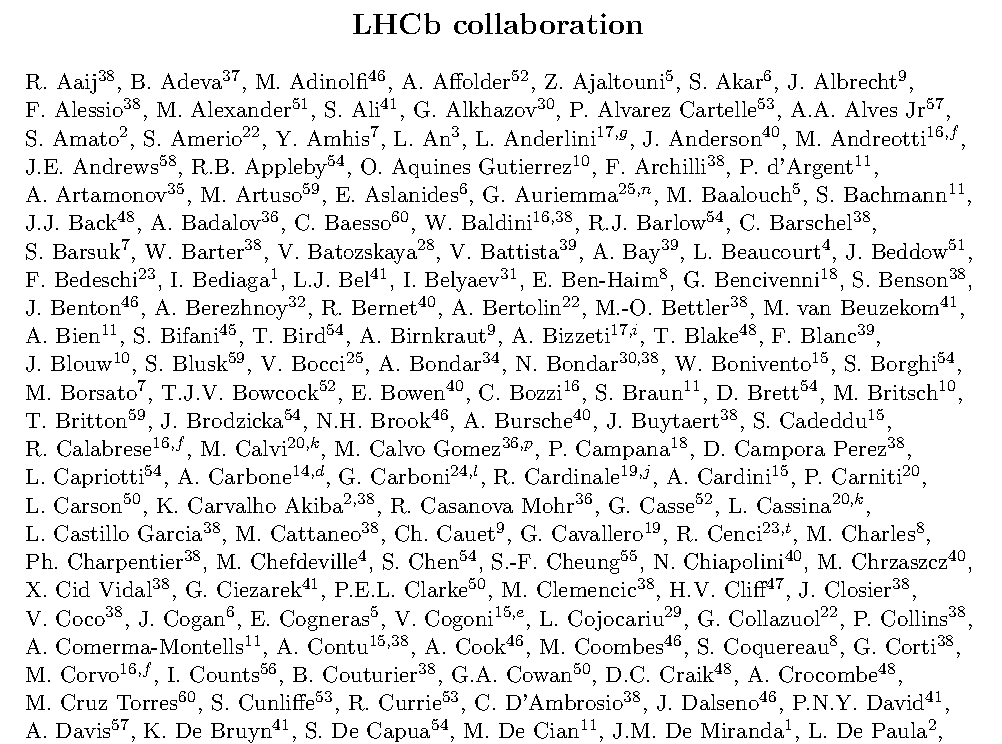
\includegraphics[width=0.45\textwidth]{Figures/authors.pdf}} & 
\subfloat[Collaboration affiliation list.]{
\includegraphics[width=0.45\textwidth]{Figures/affiliations.pdf}}\\
\end{tabular}
\caption{Figure (A) shows a collaboration field in a header section. Figure (B) shows discontinuous front matter that sits on the first page, but apart from the main header section and within the introductory section. Figures (C) and (D) give the authors list and affiliations for a large HEP collaboration; the author list begins on page 8 and continues to page 33. Figure (B) from (\cite{maguire2012taxonomy}), other excerpts from (\cite{aaij2015identification}).}
\label{fig:articlesamples}
\end{figure}
\end{frame}

%------------------------------------------------

\begin{frame}
\frametitle{}
\begin{table}[h]
\begin{center}
\begin{tabular}{|c|c|c|}
\hline
Model & HEP & CORA \\
\hline
Header & 157 papers & \textbf{2506 papers} \\
\hline
Segmentation & \textbf{169 papers} & 125 papers \\
\hline
\end{tabular}
\caption[Number of training instances for each model from each dataset.]{Number of training instances for each model from each dataset.}
\label{table:hepvscora}
\end{center}
\end{table}
\end{frame}

%------------------------------------------------

\begin{frame}
\frametitle{}
\end{frame}

%------------------------------------------------

\section{Key Results}

%------------------------------------------------

\begin{frame}[noframenumbering]{Outline}
\tableofcontents[currentsection, currentsubsection]
\end{frame}

%------------------------------------------------

\begin{frame}
\frametitle{Experiment Setup}
\end{frame}

%------------------------------------------------

\begin{frame}
\frametitle{}
\begin{figure}[h]
\center
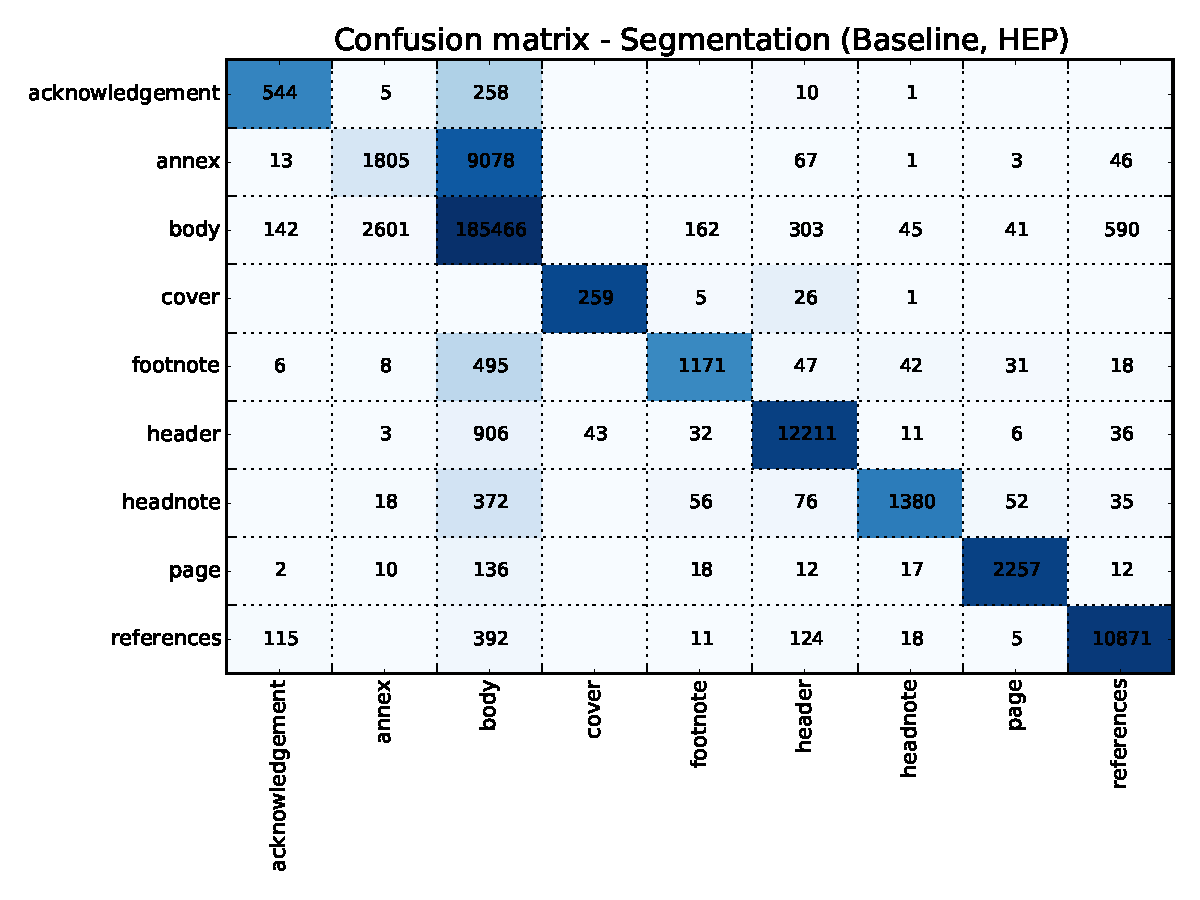
\includegraphics[width=4in]{Figures/baseline_confusion_segmentation.pdf}
\caption{Baseline confusion segmentation}
\end{figure}
\end{frame}

%------------------------------------------------

\begin{frame}
\frametitle{}
\begin{figure}[h]
\center
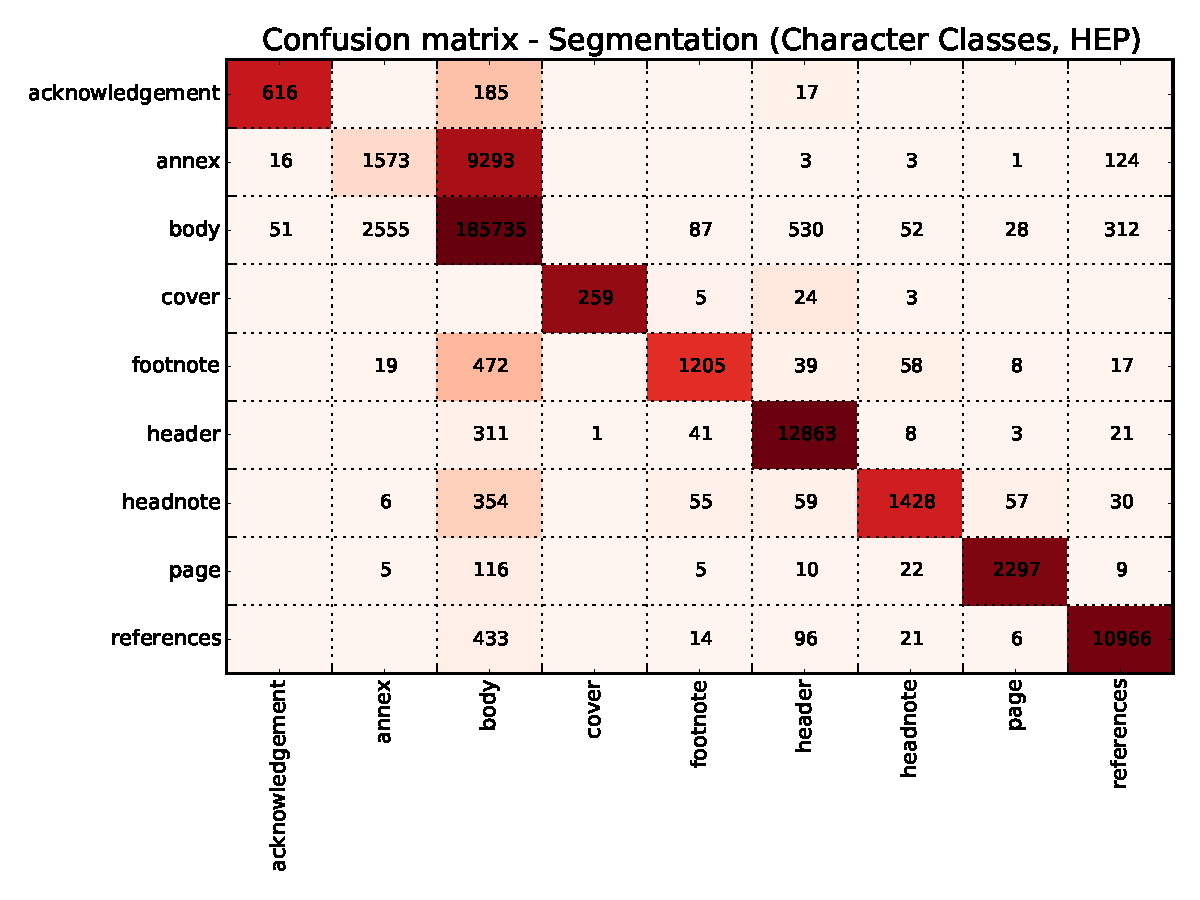
\includegraphics[width=4in]{Figures/classes_confusion_segmentation.pdf}
\caption{Classes confusion segmentation}
\end{figure}
\end{frame}

%------------------------------------------------

\begin{frame}
\frametitle{}
\end{frame}

%------------------------------------------------

\section{Conclusions}

%------------------------------------------------

\begin{frame}[noframenumbering]{Outline}
\tableofcontents[currentsection, currentsubsection]
\end{frame}

%------------------------------------------------

\begin{frame}
\frametitle{}
\end{frame}

%------------------------------------------------

\bibliographystyle{ieeetr} % Use the "unsrtnat" BibTeX style for formatting the Bibliography
\bibliography{Bibliography} % The references (bibliography) information are stored in the file named "Bibliography.bib"

\end{document} 